\documentclass[1p]{elsarticle_modified}
%\bibliographystyle{elsarticle-num}

%\usepackage[colorlinks]{hyperref}
%\usepackage{abbrmath_seonhwa} %\Abb, \Ascr, \Acal ,\Abf, \Afrak
\usepackage{amsfonts}
\usepackage{amssymb}
\usepackage{amsmath}
\usepackage{amsthm}
\usepackage{scalefnt}
\usepackage{amsbsy}
\usepackage{kotex}
\usepackage{caption}
\usepackage{subfig}
\usepackage{color}
\usepackage{graphicx}
\usepackage{xcolor} %% white, black, red, green, blue, cyan, magenta, yellow
\usepackage{float}
\usepackage{setspace}
\usepackage{hyperref}

\usepackage{tikz}
\usetikzlibrary{arrows}

\usepackage{multirow}
\usepackage{array} % fixed length table
\usepackage{hhline}

%%%%%%%%%%%%%%%%%%%%%
\makeatletter
\renewcommand*\env@matrix[1][\arraystretch]{%
	\edef\arraystretch{#1}%
	\hskip -\arraycolsep
	\let\@ifnextchar\new@ifnextchar
	\array{*\c@MaxMatrixCols c}}
\makeatother %https://tex.stackexchange.com/questions/14071/how-can-i-increase-the-line-spacing-in-a-matrix
%%%%%%%%%%%%%%%

\usepackage[normalem]{ulem}

\newcommand{\msout}[1]{\ifmmode\text{\sout{\ensuremath{#1}}}\else\sout{#1}\fi}
%SOURCE: \msout is \stkout macro in https://tex.stackexchange.com/questions/20609/strikeout-in-math-mode

\newcommand{\cancel}[1]{
	\ifmmode
	{\color{red}\msout{#1}}
	\else
	{\color{red}\sout{#1}}
	\fi
}

\newcommand{\add}[1]{
	{\color{blue}\uwave{#1}}
}

\newcommand{\replace}[2]{
	\ifmmode
	{\color{red}\msout{#1}}{\color{blue}\uwave{#2}}
	\else
	{\color{red}\sout{#1}}{\color{blue}\uwave{#2}}
	\fi
}

\newcommand{\Sol}{\mathcal{S}} %segment
\newcommand{\D}{D} %diagram
\newcommand{\A}{\mathcal{A}} %arc


%%%%%%%%%%%%%%%%%%%%%%%%%%%%%5 test

\def\sl{\operatorname{\textup{SL}}(2,\Cbb)}
\def\psl{\operatorname{\textup{PSL}}(2,\Cbb)}
\def\quan{\mkern 1mu \triangleright \mkern 1mu}

\theoremstyle{definition}
\newtheorem{thm}{Theorem}[section]
\newtheorem{prop}[thm]{Proposition}
\newtheorem{lem}[thm]{Lemma}
\newtheorem{ques}[thm]{Question}
\newtheorem{cor}[thm]{Corollary}
\newtheorem{defn}[thm]{Definition}
\newtheorem{exam}[thm]{Example}
\newtheorem{rmk}[thm]{Remark}
\newtheorem{alg}[thm]{Algorithm}

\newcommand{\I}{\sqrt{-1}}
\begin{document}

%\begin{frontmatter}
%
%\title{Boundary parabolic representations of knots up to 8 crossings}
%
%%% Group authors per affiliation:
%\author{Yunhi Cho} 
%\address{Department of Mathematics, University of Seoul, Seoul, Korea}
%\ead{yhcho@uos.ac.kr}
%
%
%\author{Seonhwa Kim} %\fnref{s_kim}}
%\address{Center for Geometry and Physics, Institute for Basic Science, Pohang, 37673, Korea}
%\ead{ryeona17@ibs.re.kr}
%
%\author{Hyuk Kim}
%\address{Department of Mathematical Sciences, Seoul National University, Seoul 08826, Korea}
%\ead{hyukkim@snu.ac.kr}
%
%\author{Seokbeom Yoon}
%\address{Department of Mathematical Sciences, Seoul National University, Seoul, 08826,  Korea}
%\ead{sbyoon15@snu.ac.kr}
%
%\begin{abstract}
%We find all boundary parabolic representation of knots up to 8 crossings.
%
%\end{abstract}
%\begin{keyword}
%    \MSC[2010] 57M25 
%\end{keyword}
%
%\end{frontmatter}

%\linenumbers
%\tableofcontents
%
\newcommand\colored[1]{\textcolor{white}{\rule[-0.35ex]{0.8em}{1.4ex}}\kern-0.8em\color{red} #1}%
%\newcommand\colored[1]{\textcolor{white}{ #1}\kern-2.17ex	\textcolor{white}{ #1}\kern-1.81ex	\textcolor{white}{ #1}\kern-2.15ex\color{red}#1	}

{\Large $\underline{12a_{0141}~(K12a_{0141})}$}

\setlength{\tabcolsep}{10pt}
\renewcommand{\arraystretch}{1.6}
\vspace{1cm}\begin{tabular}{m{100pt}>{\centering\arraybackslash}m{274pt}}
\multirow{5}{120pt}{
	\centering
	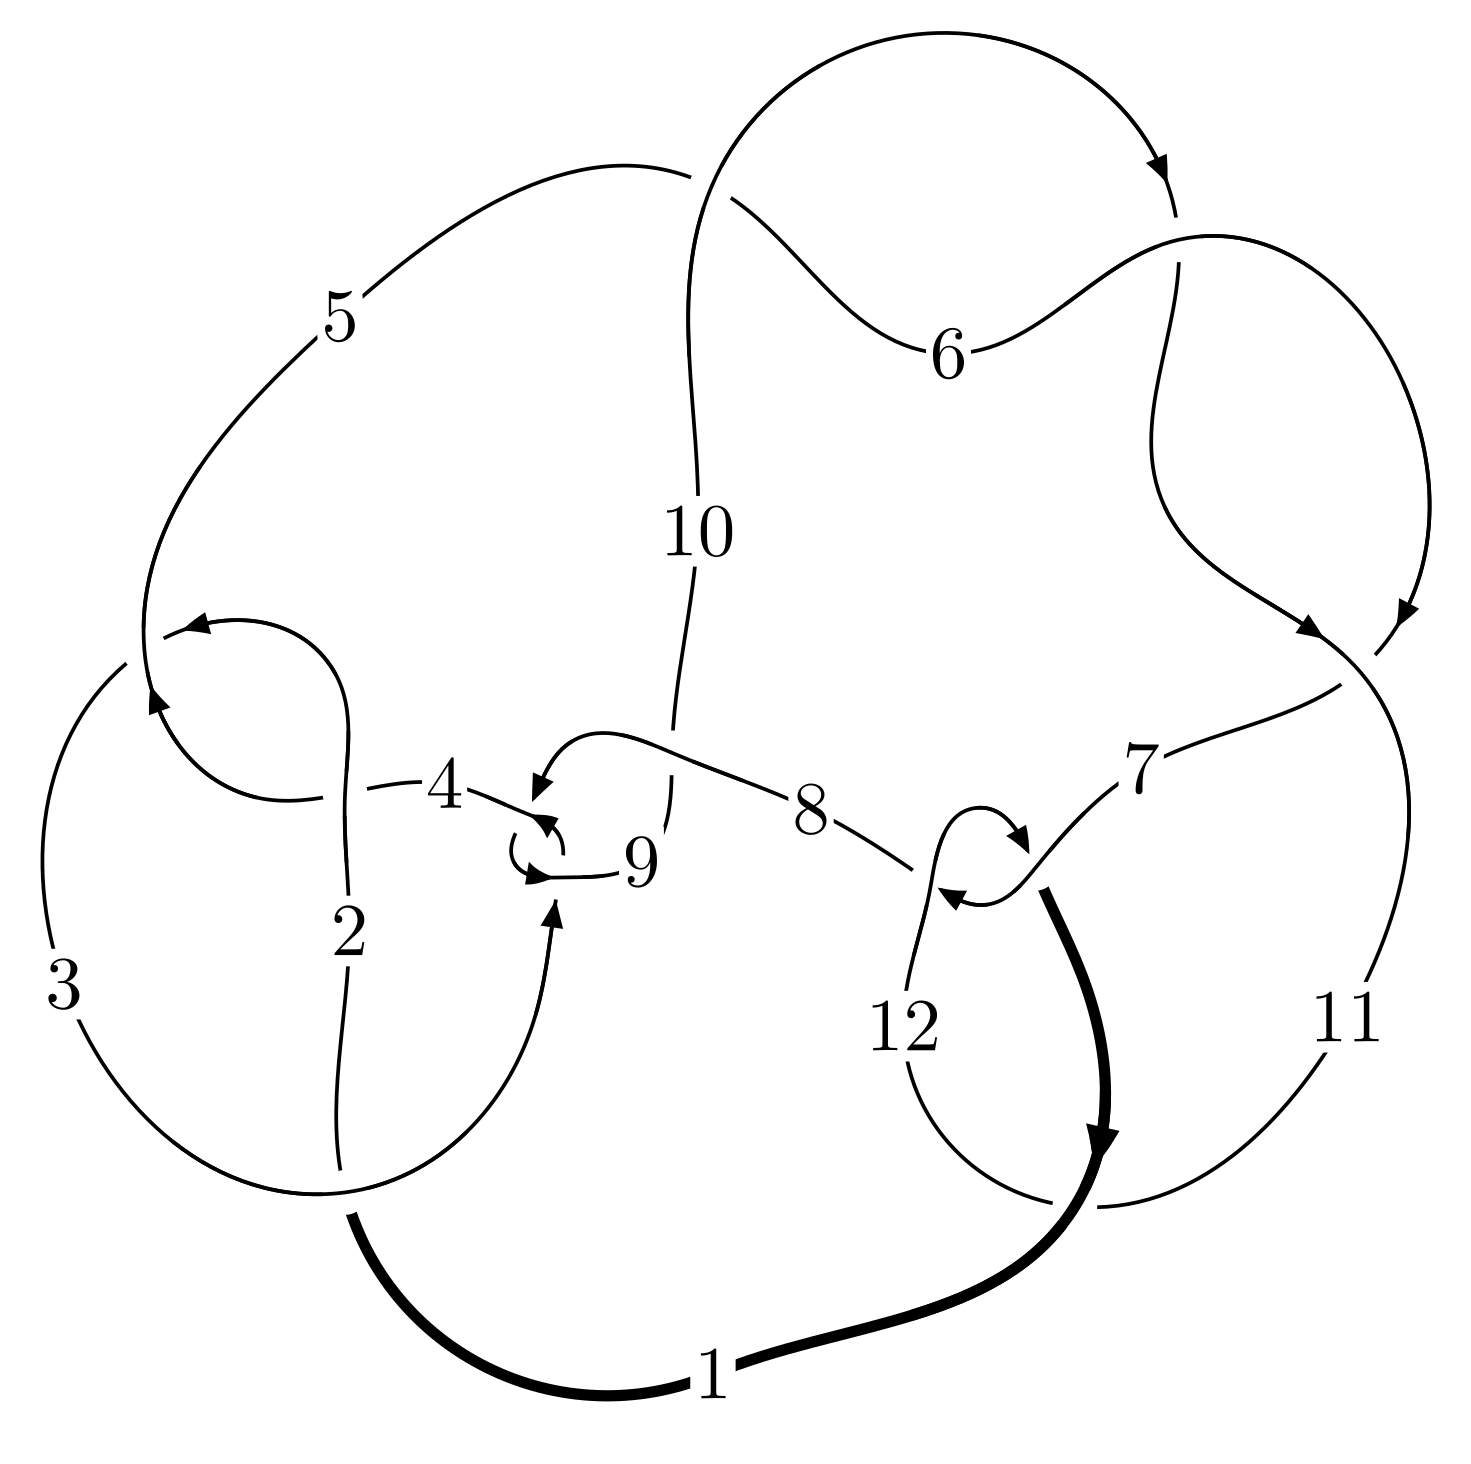
\includegraphics[width=112pt]{../../../GIT/diagram.site/Diagrams/png/942_12a_0141.png}\\
\ \ \ A knot diagram\footnotemark}&
\allowdisplaybreaks
\textbf{Linearized knot diagam} \\
\cline{2-2}
 &
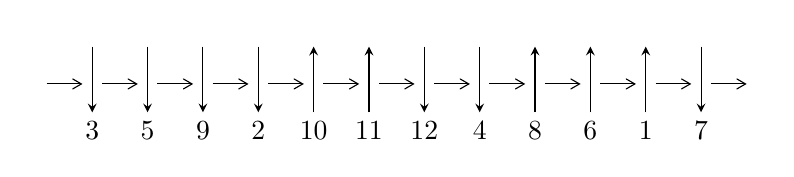
\begin{tikzpicture}[x=20pt, y=17pt]
	% nodes
	\node (C0) at (0, 0) {};
	\node (C1) at (1, 0) {};
	\node (C1U) at (1, +1) {};
	\node (C1D) at (1, -1) {3};

	\node (C2) at (2, 0) {};
	\node (C2U) at (2, +1) {};
	\node (C2D) at (2, -1) {5};

	\node (C3) at (3, 0) {};
	\node (C3U) at (3, +1) {};
	\node (C3D) at (3, -1) {9};

	\node (C4) at (4, 0) {};
	\node (C4U) at (4, +1) {};
	\node (C4D) at (4, -1) {2};

	\node (C5) at (5, 0) {};
	\node (C5U) at (5, +1) {};
	\node (C5D) at (5, -1) {10};

	\node (C6) at (6, 0) {};
	\node (C6U) at (6, +1) {};
	\node (C6D) at (6, -1) {11};

	\node (C7) at (7, 0) {};
	\node (C7U) at (7, +1) {};
	\node (C7D) at (7, -1) {12};

	\node (C8) at (8, 0) {};
	\node (C8U) at (8, +1) {};
	\node (C8D) at (8, -1) {4};

	\node (C9) at (9, 0) {};
	\node (C9U) at (9, +1) {};
	\node (C9D) at (9, -1) {8};

	\node (C10) at (10, 0) {};
	\node (C10U) at (10, +1) {};
	\node (C10D) at (10, -1) {6};

	\node (C11) at (11, 0) {};
	\node (C11U) at (11, +1) {};
	\node (C11D) at (11, -1) {1};

	\node (C12) at (12, 0) {};
	\node (C12U) at (12, +1) {};
	\node (C12D) at (12, -1) {7};
	\node (C13) at (13, 0) {};

	% arrows
	\draw[->,>={angle 60}]
	(C0) edge (C1) (C1) edge (C2) (C2) edge (C3) (C3) edge (C4) (C4) edge (C5) (C5) edge (C6) (C6) edge (C7) (C7) edge (C8) (C8) edge (C9) (C9) edge (C10) (C10) edge (C11) (C11) edge (C12) (C12) edge (C13) ;	\draw[->,>=stealth]
	(C1U) edge (C1D) (C2U) edge (C2D) (C3U) edge (C3D) (C4U) edge (C4D) (C5D) edge (C5U) (C6D) edge (C6U) (C7U) edge (C7D) (C8U) edge (C8D) (C9D) edge (C9U) (C10D) edge (C10U) (C11D) edge (C11U) (C12U) edge (C12D) ;
	\end{tikzpicture} \\
\hhline{~~} \\& 
\textbf{Solving Sequence} \\ \cline{2-2} 
 &
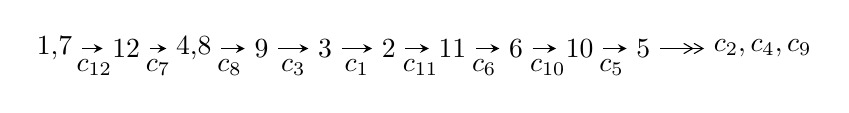
\begin{tikzpicture}[x=23pt, y=7pt]
	% node
	\node (A0) at (-1/8, 0) {1,7};
	\node (A1) at (1, 0) {12};
	\node (A2) at (33/16, 0) {4,8};
	\node (A3) at (25/8, 0) {9};
	\node (A4) at (33/8, 0) {3};
	\node (A5) at (41/8, 0) {2};
	\node (A6) at (49/8, 0) {11};
	\node (A7) at (57/8, 0) {6};
	\node (A8) at (65/8, 0) {10};
	\node (A9) at (73/8, 0) {5};
	\node (C1) at (1/2, -1) {$c_{12}$};
	\node (C2) at (3/2, -1) {$c_{7}$};
	\node (C3) at (21/8, -1) {$c_{8}$};
	\node (C4) at (29/8, -1) {$c_{3}$};
	\node (C5) at (37/8, -1) {$c_{1}$};
	\node (C6) at (45/8, -1) {$c_{11}$};
	\node (C7) at (53/8, -1) {$c_{6}$};
	\node (C8) at (61/8, -1) {$c_{10}$};
	\node (C9) at (69/8, -1) {$c_{5}$};
	\node (A10) at (11, 0) {$c_{2},c_{4},c_{9}$};

	% edge
	\draw[->,>=stealth]	
	(A0) edge (A1) (A1) edge (A2) (A2) edge (A3) (A3) edge (A4) (A4) edge (A5) (A5) edge (A6) (A6) edge (A7) (A7) edge (A8) (A8) edge (A9) ;
	\draw[->>,>={angle 60}]	
	(A9) edge (A10);
\end{tikzpicture} \\ 

\end{tabular} \\

\footnotetext{
The image of knot diagram is generated by the software ``\textbf{Draw programme}" developed by Andrew Bartholomew(\url{http://www.layer8.co.uk/maths/draw/index.htm\#Running-draw}), where we modified some parts for our purpose(\url{https://github.com/CATsTAILs/LinksPainter}).
}\phantom \\ \newline 
\centering \textbf{Ideals for irreducible components\footnotemark of $X_{\text{par}}$} 
 
\begin{align*}
I^u_{1}&=\langle 
- u^{83}- u^{82}+\cdots+b-3 u,\;- u^{83}- u^{82}+\cdots+a+1,\;u^{85}+2 u^{84}+\cdots+3 u+1\rangle \\
I^u_{2}&=\langle 
b-1,\;u^3- u^2+a+u,\;u^5- u^4+2 u^3- u^2+u-1\rangle \\
\\
\end{align*}
\raggedright * 2 irreducible components of $\dim_{\mathbb{C}}=0$, with total 90 representations.\\
\footnotetext{All coefficients of polynomials are rational numbers. But the coefficients are sometimes approximated in decimal forms when there is not enough margin.}
\newpage
\renewcommand{\arraystretch}{1}
\centering \section*{I. $I^u_{1}= \langle - u^{83}- u^{82}+\cdots+b-3 u,\;- u^{83}- u^{82}+\cdots+a+1,\;u^{85}+2 u^{84}+\cdots+3 u+1 \rangle$}
\flushleft \textbf{(i) Arc colorings}\\
\begin{tabular}{m{7pt} m{180pt} m{7pt} m{180pt} }
\flushright $a_{1}=$&$\begin{pmatrix}1\\0\end{pmatrix}$ \\
\flushright $a_{7}=$&$\begin{pmatrix}0\\u\end{pmatrix}$ \\
\flushright $a_{12}=$&$\begin{pmatrix}1\\- u^2\end{pmatrix}$ \\
\flushright $a_{4}=$&$\begin{pmatrix}u^{83}+u^{82}+\cdots-2 u^2-1\\u^{83}+u^{82}+\cdots- u^3+3 u\end{pmatrix}$ \\
\flushright $a_{8}=$&$\begin{pmatrix}- u\\u^3+u\end{pmatrix}$ \\
\flushright $a_{9}=$&$\begin{pmatrix}u^{12}+3 u^{10}+3 u^8-2 u^6-4 u^4- u^2+1\\- u^{14}-4 u^{12}-7 u^{10}-4 u^8+2 u^6+4 u^4+u^2\end{pmatrix}$ \\
\flushright $a_{3}=$&$\begin{pmatrix}- u^{83}- u^{82}+\cdots- u-2\\u^{83}+u^{82}+\cdots-2 u^2+2 u\end{pmatrix}$ \\
\flushright $a_{2}=$&$\begin{pmatrix}u^{81}+u^{80}+\cdots+2 u^2+2\\- u^{83}- u^{82}+\cdots- u^3-2 u\end{pmatrix}$ \\
\flushright $a_{11}=$&$\begin{pmatrix}u^2+1\\- u^2\end{pmatrix}$ \\
\flushright $a_{6}=$&$\begin{pmatrix}- u^5-2 u^3- u\\u^5+u^3+u\end{pmatrix}$ \\
\flushright $a_{10}=$&$\begin{pmatrix}- u^8-3 u^6-3 u^4+1\\u^8+2 u^6+2 u^4\end{pmatrix}$ \\
\flushright $a_{5}=$&$\begin{pmatrix}u^{11}+4 u^9+6 u^7+2 u^5-3 u^3-2 u\\- u^{11}-3 u^9-4 u^7- u^5+u^3+u\end{pmatrix}$\\&\end{tabular}
\flushleft \textbf{(ii) Obstruction class $= -1$}\\~\\
\flushleft \textbf{(iii) Cusp Shapes $= -4 u^{84}-3 u^{83}+\cdots-19 u^2-7$}\\~\\
\newpage\renewcommand{\arraystretch}{1}
\flushleft \textbf{(iv) u-Polynomials at the component}\newline \\
\begin{tabular}{m{50pt}|m{274pt}}
Crossings & \hspace{64pt}u-Polynomials at each crossing \\
\hline $$\begin{aligned}c_{1}\end{aligned}$$&$\begin{aligned}
&u^{85}+44 u^{84}+\cdots+5 u+1
\end{aligned}$\\
\hline $$\begin{aligned}c_{2},c_{4}\end{aligned}$$&$\begin{aligned}
&u^{85}-6 u^{84}+\cdots-7 u+1
\end{aligned}$\\
\hline $$\begin{aligned}c_{3},c_{8}\end{aligned}$$&$\begin{aligned}
&u^{85}- u^{84}+\cdots+280 u^2+32
\end{aligned}$\\
\hline $$\begin{aligned}c_{5},c_{6},c_{10}\end{aligned}$$&$\begin{aligned}
&u^{85}-2 u^{84}+\cdots+69 u+9
\end{aligned}$\\
\hline $$\begin{aligned}c_{7},c_{12}\end{aligned}$$&$\begin{aligned}
&u^{85}+2 u^{84}+\cdots+3 u+1
\end{aligned}$\\
\hline $$\begin{aligned}c_{9}\end{aligned}$$&$\begin{aligned}
&u^{85}-33 u^{84}+\cdots-17920 u+1024
\end{aligned}$\\
\hline $$\begin{aligned}c_{11}\end{aligned}$$&$\begin{aligned}
&u^{85}-48 u^{84}+\cdots+11 u+1
\end{aligned}$\\
\hline
\end{tabular}\\~\\
\newpage\renewcommand{\arraystretch}{1}
\flushleft \textbf{(v) Riley Polynomials at the component}\newline \\
\begin{tabular}{m{50pt}|m{274pt}}
Crossings & \hspace{64pt}Riley Polynomials at each crossing \\
\hline $$\begin{aligned}c_{1}\end{aligned}$$&$\begin{aligned}
&y^{85}+68 y^{83}+\cdots+29 y-1
\end{aligned}$\\
\hline $$\begin{aligned}c_{2},c_{4}\end{aligned}$$&$\begin{aligned}
&y^{85}-44 y^{84}+\cdots+5 y-1
\end{aligned}$\\
\hline $$\begin{aligned}c_{3},c_{8}\end{aligned}$$&$\begin{aligned}
&y^{85}+33 y^{84}+\cdots-17920 y-1024
\end{aligned}$\\
\hline $$\begin{aligned}c_{5},c_{6},c_{10}\end{aligned}$$&$\begin{aligned}
&y^{85}-88 y^{84}+\cdots+5643 y-81
\end{aligned}$\\
\hline $$\begin{aligned}c_{7},c_{12}\end{aligned}$$&$\begin{aligned}
&y^{85}+48 y^{84}+\cdots+11 y-1
\end{aligned}$\\
\hline $$\begin{aligned}c_{9}\end{aligned}$$&$\begin{aligned}
&y^{85}+29 y^{84}+\cdots+17432576 y-1048576
\end{aligned}$\\
\hline $$\begin{aligned}c_{11}\end{aligned}$$&$\begin{aligned}
&y^{85}-20 y^{84}+\cdots+283 y-1
\end{aligned}$\\
\hline
\end{tabular}\\~\\
\newpage\flushleft \textbf{(vi) Complex Volumes and Cusp Shapes}
$$\begin{array}{c|c|c}  
\text{Solutions to }I^u_{1}& \I (\text{vol} + \sqrt{-1}CS) & \text{Cusp shape}\\
 \hline 
\begin{aligned}
u &= -0.427067 + 0.903288 I \\
a &= -1.45806 + 0.54783 I \\
b &= -0.093443 - 0.592929 I\end{aligned}
 & \phantom{-}0.15850 + 2.06285 I & \phantom{-0.000000 } 0 \\ \hline\begin{aligned}
u &= -0.427067 - 0.903288 I \\
a &= -1.45806 - 0.54783 I \\
b &= -0.093443 + 0.592929 I\end{aligned}
 & \phantom{-}0.15850 - 2.06285 I & \phantom{-0.000000 } 0 \\ \hline\begin{aligned}
u &= -0.299920 + 0.963143 I \\
a &= -0.70616 + 1.28928 I \\
b &= -0.444864 + 0.101720 I\end{aligned}
 & \phantom{-}0.80832 + 2.36710 I & \phantom{-0.000000 } 0 \\ \hline\begin{aligned}
u &= -0.299920 - 0.963143 I \\
a &= -0.70616 - 1.28928 I \\
b &= -0.444864 - 0.101720 I\end{aligned}
 & \phantom{-}0.80832 - 2.36710 I & \phantom{-0.000000 } 0 \\ \hline\begin{aligned}
u &= -0.515060 + 0.884059 I \\
a &= \phantom{-}2.20223 - 0.11337 I \\
b &= -0.489025 + 1.097400 I\end{aligned}
 & -2.47171 - 1.64225 I & \phantom{-0.000000 } 0 \\ \hline\begin{aligned}
u &= -0.515060 - 0.884059 I \\
a &= \phantom{-}2.20223 + 0.11337 I \\
b &= -0.489025 - 1.097400 I\end{aligned}
 & -2.47171 + 1.64225 I & \phantom{-0.000000 } 0 \\ \hline\begin{aligned}
u &= -0.127090 + 0.966533 I \\
a &= \phantom{-}0.14971 - 1.50302 I \\
b &= -0.162922 - 0.575892 I\end{aligned}
 & -0.189918 - 0.769631 I & \phantom{-0.000000 } 0 \\ \hline\begin{aligned}
u &= -0.127090 - 0.966533 I \\
a &= \phantom{-}0.14971 + 1.50302 I \\
b &= -0.162922 + 0.575892 I\end{aligned}
 & -0.189918 + 0.769631 I & \phantom{-0.000000 } 0 \\ \hline\begin{aligned}
u &= \phantom{-}0.472646 + 0.937491 I \\
a &= -1.30201 - 2.40692 I \\
b &= -0.75331 + 1.77642 I\end{aligned}
 & -2.91281 - 3.22612 I & \phantom{-0.000000 } 0 \\ \hline\begin{aligned}
u &= \phantom{-}0.472646 - 0.937491 I \\
a &= -1.30201 + 2.40692 I \\
b &= -0.75331 - 1.77642 I\end{aligned}
 & -2.91281 + 3.22612 I & \phantom{-0.000000 } 0\\
 \hline 
 \end{array}$$\newpage$$\begin{array}{c|c|c}  
\text{Solutions to }I^u_{1}& \I (\text{vol} + \sqrt{-1}CS) & \text{Cusp shape}\\
 \hline 
\begin{aligned}
u &= \phantom{-}0.148743 + 1.053900 I \\
a &= \phantom{-}0.031322 + 0.766541 I \\
b &= \phantom{-}1.145100 + 0.559030 I\end{aligned}
 & \phantom{-}3.86682 + 1.00502 I & \phantom{-0.000000 } 0 \\ \hline\begin{aligned}
u &= \phantom{-}0.148743 - 1.053900 I \\
a &= \phantom{-}0.031322 - 0.766541 I \\
b &= \phantom{-}1.145100 - 0.559030 I\end{aligned}
 & \phantom{-}3.86682 - 1.00502 I & \phantom{-0.000000 } 0 \\ \hline\begin{aligned}
u &= -0.482726 + 0.958907 I \\
a &= \phantom{-}2.09417 - 0.93018 I \\
b &= \phantom{-}0.361332 + 1.235000 I\end{aligned}
 & -2.60128 + 5.81097 I & \phantom{-0.000000 } 0 \\ \hline\begin{aligned}
u &= -0.482726 - 0.958907 I \\
a &= \phantom{-}2.09417 + 0.93018 I \\
b &= \phantom{-}0.361332 - 1.235000 I\end{aligned}
 & -2.60128 - 5.81097 I & \phantom{-0.000000 } 0 \\ \hline\begin{aligned}
u &= \phantom{-}0.094327 + 1.083490 I \\
a &= -0.282344 - 1.027780 I \\
b &= -1.192310 - 0.747964 I\end{aligned}
 & \phantom{-}1.72458 + 5.87992 I & \phantom{-0.000000 } 0 \\ \hline\begin{aligned}
u &= \phantom{-}0.094327 - 1.083490 I \\
a &= -0.282344 + 1.027780 I \\
b &= -1.192310 + 0.747964 I\end{aligned}
 & \phantom{-}1.72458 - 5.87992 I & \phantom{-0.000000 } 0 \\ \hline\begin{aligned}
u &= \phantom{-}0.221914 + 0.883158 I \\
a &= \phantom{-}1.20820 - 1.44716 I \\
b &= -1.45625 - 0.47093 I\end{aligned}
 & -0.855582 - 1.085530 I & \phantom{-}4.15462 - 1.86707 I \\ \hline\begin{aligned}
u &= \phantom{-}0.221914 - 0.883158 I \\
a &= \phantom{-}1.20820 + 1.44716 I \\
b &= -1.45625 + 0.47093 I\end{aligned}
 & -0.855582 + 1.085530 I & \phantom{-}4.15462 + 1.86707 I \\ \hline\begin{aligned}
u &= \phantom{-}0.488530 + 0.986861 I \\
a &= \phantom{-}0.70570 + 2.33378 I \\
b &= \phantom{-}1.01921 - 1.22307 I\end{aligned}
 & \phantom{-}1.47835 - 6.73642 I & \phantom{-0.000000 } 0 \\ \hline\begin{aligned}
u &= \phantom{-}0.488530 - 0.986861 I \\
a &= \phantom{-}0.70570 - 2.33378 I \\
b &= \phantom{-}1.01921 + 1.22307 I\end{aligned}
 & \phantom{-}1.47835 + 6.73642 I & \phantom{-0.000000 } 0\\
 \hline 
 \end{array}$$\newpage$$\begin{array}{c|c|c}  
\text{Solutions to }I^u_{1}& \I (\text{vol} + \sqrt{-1}CS) & \text{Cusp shape}\\
 \hline 
\begin{aligned}
u &= \phantom{-}0.517691 + 0.981760 I \\
a &= -0.62999 - 2.67424 I \\
b &= -1.38554 + 1.33578 I\end{aligned}
 & -1.25752 - 11.69060 I & \phantom{-0.000000 } 0 \\ \hline\begin{aligned}
u &= \phantom{-}0.517691 - 0.981760 I \\
a &= -0.62999 + 2.67424 I \\
b &= -1.38554 - 1.33578 I\end{aligned}
 & -1.25752 + 11.69060 I & \phantom{-0.000000 } 0 \\ \hline\begin{aligned}
u &= -0.429195 + 0.777445 I \\
a &= -1.174550 - 0.530055 I \\
b &= \phantom{-}0.415792 - 0.088181 I\end{aligned}
 & -0.06950 + 1.83366 I & \phantom{-}0.66649 - 5.14350 I \\ \hline\begin{aligned}
u &= -0.429195 - 0.777445 I \\
a &= -1.174550 + 0.530055 I \\
b &= \phantom{-}0.415792 + 0.088181 I\end{aligned}
 & -0.06950 - 1.83366 I & \phantom{-}0.66649 + 5.14350 I \\ \hline\begin{aligned}
u &= \phantom{-}0.290125 + 1.079680 I \\
a &= -0.170641 - 0.295666 I \\
b &= \phantom{-}0.738944 + 0.278480 I\end{aligned}
 & \phantom{-}5.05386 - 1.05004 I & \phantom{-0.000000 } 0 \\ \hline\begin{aligned}
u &= \phantom{-}0.290125 - 1.079680 I \\
a &= -0.170641 + 0.295666 I \\
b &= \phantom{-}0.738944 - 0.278480 I\end{aligned}
 & \phantom{-}5.05386 + 1.05004 I & \phantom{-0.000000 } 0 \\ \hline\begin{aligned}
u &= -0.872592 + 0.011682 I \\
a &= -0.13799 + 1.46426 I \\
b &= \phantom{-}0.319385 - 1.125930 I\end{aligned}
 & \phantom{-}9.16696 - 2.75702 I & \phantom{-}3.57442 + 3.01021 I \\ \hline\begin{aligned}
u &= -0.872592 - 0.011682 I \\
a &= -0.13799 - 1.46426 I \\
b &= \phantom{-}0.319385 + 1.125930 I\end{aligned}
 & \phantom{-}9.16696 + 2.75702 I & \phantom{-}3.57442 - 3.01021 I \\ \hline\begin{aligned}
u &= -0.863233 + 0.080625 I \\
a &= \phantom{-}0.81138 - 1.42675 I \\
b &= -1.91866 + 1.20507 I\end{aligned}
 & \phantom{-}3.48230 - 11.13990 I & -1.12808 + 7.06717 I \\ \hline\begin{aligned}
u &= -0.863233 - 0.080625 I \\
a &= \phantom{-}0.81138 + 1.42675 I \\
b &= -1.91866 - 1.20507 I\end{aligned}
 & \phantom{-}3.48230 + 11.13990 I & -1.12808 - 7.06717 I\\
 \hline 
 \end{array}$$\newpage$$\begin{array}{c|c|c}  
\text{Solutions to }I^u_{1}& \I (\text{vol} + \sqrt{-1}CS) & \text{Cusp shape}\\
 \hline 
\begin{aligned}
u &= -0.860540 + 0.064517 I \\
a &= -0.70023 + 1.48083 I \\
b &= \phantom{-}1.62593 - 1.28684 I\end{aligned}
 & \phantom{-}6.12444 - 5.75564 I & \phantom{-}2.12476 + 3.50801 I \\ \hline\begin{aligned}
u &= -0.860540 - 0.064517 I \\
a &= -0.70023 - 1.48083 I \\
b &= \phantom{-}1.62593 + 1.28684 I\end{aligned}
 & \phantom{-}6.12444 + 5.75564 I & \phantom{-}2.12476 - 3.50801 I \\ \hline\begin{aligned}
u &= \phantom{-}0.844152 + 0.062878 I \\
a &= \phantom{-}0.268712 - 0.119606 I \\
b &= \phantom{-}0.752344 + 0.745016 I\end{aligned}
 & \phantom{-}1.62409 + 4.88126 I & -2.48263 - 3.81093 I \\ \hline\begin{aligned}
u &= \phantom{-}0.844152 - 0.062878 I \\
a &= \phantom{-}0.268712 + 0.119606 I \\
b &= \phantom{-}0.752344 - 0.745016 I\end{aligned}
 & \phantom{-}1.62409 - 4.88126 I & -2.48263 + 3.81093 I \\ \hline\begin{aligned}
u &= \phantom{-}0.388889 + 1.096620 I \\
a &= \phantom{-}0.099797 + 0.999827 I \\
b &= -0.0317490 - 0.1256150 I\end{aligned}
 & \phantom{-}4.33398 - 5.66355 I & \phantom{-0.000000 } 0 \\ \hline\begin{aligned}
u &= \phantom{-}0.388889 - 1.096620 I \\
a &= \phantom{-}0.099797 - 0.999827 I \\
b &= -0.0317490 + 0.1256150 I\end{aligned}
 & \phantom{-}4.33398 + 5.66355 I & \phantom{-0.000000 } 0 \\ \hline\begin{aligned}
u &= -0.831465 + 0.054925 I \\
a &= \phantom{-}0.75430 - 1.75204 I \\
b &= -1.62680 + 1.91695 I\end{aligned}
 & \phantom{-}0.96832 - 2.23146 I & -2.03853 + 3.04442 I \\ \hline\begin{aligned}
u &= -0.831465 - 0.054925 I \\
a &= \phantom{-}0.75430 + 1.75204 I \\
b &= -1.62680 - 1.91695 I\end{aligned}
 & \phantom{-}0.96832 + 2.23146 I & -2.03853 - 3.04442 I \\ \hline\begin{aligned}
u &= \phantom{-}0.829680 + 0.029626 I \\
a &= -0.212091 + 0.030369 I \\
b &= -0.707910 - 0.329097 I\end{aligned}
 & \phantom{-}3.58523 + 0.53976 I & \phantom{-}0.236036 + 1.036399 I \\ \hline\begin{aligned}
u &= \phantom{-}0.829680 - 0.029626 I \\
a &= -0.212091 - 0.030369 I \\
b &= -0.707910 + 0.329097 I\end{aligned}
 & \phantom{-}3.58523 - 0.53976 I & \phantom{-}0.236036 - 1.036399 I\\
 \hline 
 \end{array}$$\newpage$$\begin{array}{c|c|c}  
\text{Solutions to }I^u_{1}& \I (\text{vol} + \sqrt{-1}CS) & \text{Cusp shape}\\
 \hline 
\begin{aligned}
u &= -0.549150 + 0.588273 I \\
a &= \phantom{-}1.10721 + 1.72614 I \\
b &= -0.755841 - 1.170040 I\end{aligned}
 & -3.29788 + 5.93867 I & -5.94323 - 6.90497 I \\ \hline\begin{aligned}
u &= -0.549150 - 0.588273 I \\
a &= \phantom{-}1.10721 - 1.72614 I \\
b &= -0.755841 + 1.170040 I\end{aligned}
 & -3.29788 - 5.93867 I & -5.94323 + 6.90497 I \\ \hline\begin{aligned}
u &= \phantom{-}0.767403 + 0.105507 I \\
a &= \phantom{-}0.514337 + 0.150139 I \\
b &= -0.047203 + 0.669447 I\end{aligned}
 & \phantom{-}0.74936 - 1.67557 I & -1.83419 + 4.19037 I \\ \hline\begin{aligned}
u &= \phantom{-}0.767403 - 0.105507 I \\
a &= \phantom{-}0.514337 - 0.150139 I \\
b &= -0.047203 - 0.669447 I\end{aligned}
 & \phantom{-}0.74936 + 1.67557 I & -1.83419 - 4.19037 I \\ \hline\begin{aligned}
u &= \phantom{-}0.418759 + 1.172800 I \\
a &= -0.159145 + 0.894091 I \\
b &= \phantom{-}0.135953 + 0.365111 I\end{aligned}
 & \phantom{-}4.44095 - 5.64736 I & \phantom{-0.000000 } 0 \\ \hline\begin{aligned}
u &= \phantom{-}0.418759 - 1.172800 I \\
a &= -0.159145 - 0.894091 I \\
b &= \phantom{-}0.135953 - 0.365111 I\end{aligned}
 & \phantom{-}4.44095 + 5.64736 I & \phantom{-0.000000 } 0 \\ \hline\begin{aligned}
u &= -0.457326 + 0.591105 I \\
a &= -0.94785 - 1.41236 I \\
b &= \phantom{-}0.377468 + 0.777654 I\end{aligned}
 & -0.68556 + 1.70417 I & -2.97415 - 3.79810 I \\ \hline\begin{aligned}
u &= -0.457326 - 0.591105 I \\
a &= -0.94785 + 1.41236 I \\
b &= \phantom{-}0.377468 - 0.777654 I\end{aligned}
 & -0.68556 - 1.70417 I & -2.97415 + 3.79810 I \\ \hline\begin{aligned}
u &= \phantom{-}0.595689 + 0.441663 I \\
a &= \phantom{-}1.83391 + 1.66748 I \\
b &= -1.15659 - 1.23971 I\end{aligned}
 & -2.76956 + 7.29426 I & -5.22729 - 5.96862 I \\ \hline\begin{aligned}
u &= \phantom{-}0.595689 - 0.441663 I \\
a &= \phantom{-}1.83391 - 1.66748 I \\
b &= -1.15659 + 1.23971 I\end{aligned}
 & -2.76956 - 7.29426 I & -5.22729 + 5.96862 I\\
 \hline 
 \end{array}$$\newpage$$\begin{array}{c|c|c}  
\text{Solutions to }I^u_{1}& \I (\text{vol} + \sqrt{-1}CS) & \text{Cusp shape}\\
 \hline 
\begin{aligned}
u &= \phantom{-}0.487621 + 1.191850 I \\
a &= \phantom{-}1.067100 - 0.424092 I \\
b &= \phantom{-}0.121066 - 0.748933 I\end{aligned}
 & \phantom{-}3.93138 - 2.95603 I & \phantom{-0.000000 } 0 \\ \hline\begin{aligned}
u &= \phantom{-}0.487621 - 1.191850 I \\
a &= \phantom{-}1.067100 + 0.424092 I \\
b &= \phantom{-}0.121066 + 0.748933 I\end{aligned}
 & \phantom{-}3.93138 + 2.95603 I & \phantom{-0.000000 } 0 \\ \hline\begin{aligned}
u &= \phantom{-}0.490907 + 0.508135 I \\
a &= \phantom{-}1.56014 + 2.20056 I \\
b &= -0.40694 - 1.54213 I\end{aligned}
 & -4.10374 - 0.78290 I & -8.23718 + 0.26691 I \\ \hline\begin{aligned}
u &= \phantom{-}0.490907 - 0.508135 I \\
a &= \phantom{-}1.56014 - 2.20056 I \\
b &= -0.40694 + 1.54213 I\end{aligned}
 & -4.10374 + 0.78290 I & -8.23718 - 0.26691 I \\ \hline\begin{aligned}
u &= -0.432592 + 1.231440 I \\
a &= \phantom{-}0.76495 + 1.44194 I \\
b &= -1.82893 + 1.84485 I\end{aligned}
 & \phantom{-}4.81532 + 2.20135 I & \phantom{-0.000000 } 0 \\ \hline\begin{aligned}
u &= -0.432592 - 1.231440 I \\
a &= \phantom{-}0.76495 - 1.44194 I \\
b &= -1.82893 - 1.84485 I\end{aligned}
 & \phantom{-}4.81532 - 2.20135 I & \phantom{-0.000000 } 0 \\ \hline\begin{aligned}
u &= \phantom{-}0.445663 + 1.230960 I \\
a &= -0.581637 - 0.898159 I \\
b &= -0.761101 - 0.242276 I\end{aligned}
 & \phantom{-}7.34340 - 3.97545 I & \phantom{-0.000000 } 0 \\ \hline\begin{aligned}
u &= \phantom{-}0.445663 - 1.230960 I \\
a &= -0.581637 + 0.898159 I \\
b &= -0.761101 + 0.242276 I\end{aligned}
 & \phantom{-}7.34340 + 3.97545 I & \phantom{-0.000000 } 0 \\ \hline\begin{aligned}
u &= -0.512165 + 0.463031 I \\
a &= \phantom{-}0.63934 + 1.63821 I \\
b &= \phantom{-}0.036905 - 1.325170 I\end{aligned}
 & -3.96910 - 1.72223 I & -7.92428 + 1.16968 I \\ \hline\begin{aligned}
u &= -0.512165 - 0.463031 I \\
a &= \phantom{-}0.63934 - 1.63821 I \\
b &= \phantom{-}0.036905 + 1.325170 I\end{aligned}
 & -3.96910 + 1.72223 I & -7.92428 - 1.16968 I\\
 \hline 
 \end{array}$$\newpage$$\begin{array}{c|c|c}  
\text{Solutions to }I^u_{1}& \I (\text{vol} + \sqrt{-1}CS) & \text{Cusp shape}\\
 \hline 
\begin{aligned}
u &= \phantom{-}0.427548 + 1.238760 I \\
a &= \phantom{-}0.382640 + 1.176150 I \\
b &= \phantom{-}0.746159 + 0.605982 I\end{aligned}
 & \phantom{-}5.54728 + 0.43357 I & \phantom{-0.000000 } 0 \\ \hline\begin{aligned}
u &= \phantom{-}0.427548 - 1.238760 I \\
a &= \phantom{-}0.382640 - 1.176150 I \\
b &= \phantom{-}0.746159 - 0.605982 I\end{aligned}
 & \phantom{-}5.54728 - 0.43357 I & \phantom{-0.000000 } 0 \\ \hline\begin{aligned}
u &= \phantom{-}0.474420 + 1.224890 I \\
a &= -1.072410 - 0.442407 I \\
b &= -0.780878 + 0.397385 I\end{aligned}
 & \phantom{-}7.13458 - 5.22782 I & \phantom{-0.000000 } 0 \\ \hline\begin{aligned}
u &= \phantom{-}0.474420 - 1.224890 I \\
a &= -1.072410 + 0.442407 I \\
b &= -0.780878 - 0.397385 I\end{aligned}
 & \phantom{-}7.13458 + 5.22782 I & \phantom{-0.000000 } 0 \\ \hline\begin{aligned}
u &= -0.484834 + 1.222640 I \\
a &= -2.19593 + 1.58462 I \\
b &= -1.65391 - 2.09380 I\end{aligned}
 & \phantom{-}4.43882 + 6.98841 I & \phantom{-0.000000 } 0 \\ \hline\begin{aligned}
u &= -0.484834 - 1.222640 I \\
a &= -2.19593 - 1.58462 I \\
b &= -1.65391 + 2.09380 I\end{aligned}
 & \phantom{-}4.43882 - 6.98841 I & \phantom{-0.000000 } 0 \\ \hline\begin{aligned}
u &= -0.416514 + 1.251400 I \\
a &= -0.163665 + 1.195830 I \\
b &= -1.97265 + 1.08672 I\end{aligned}
 & \phantom{-}7.54683 - 6.68500 I & \phantom{-0.000000 } 0 \\ \hline\begin{aligned}
u &= -0.416514 - 1.251400 I \\
a &= -0.163665 - 1.195830 I \\
b &= -1.97265 - 1.08672 I\end{aligned}
 & \phantom{-}7.54683 + 6.68500 I & \phantom{-0.000000 } 0 \\ \hline\begin{aligned}
u &= -0.426785 + 1.249060 I \\
a &= -0.122637 - 1.014800 I \\
b &= \phantom{-}1.72547 - 1.20199 I\end{aligned}
 & \phantom{-}10.11510 - 1.25157 I & \phantom{-0.000000 } 0 \\ \hline\begin{aligned}
u &= -0.426785 - 1.249060 I \\
a &= -0.122637 + 1.014800 I \\
b &= \phantom{-}1.72547 + 1.20199 I\end{aligned}
 & \phantom{-}10.11510 + 1.25157 I & \phantom{-0.000000 } 0\\
 \hline 
 \end{array}$$\newpage$$\begin{array}{c|c|c}  
\text{Solutions to }I^u_{1}& \I (\text{vol} + \sqrt{-1}CS) & \text{Cusp shape}\\
 \hline 
\begin{aligned}
u &= \phantom{-}0.490124 + 1.226340 I \\
a &= \phantom{-}1.43483 + 0.30890 I \\
b &= \phantom{-}0.866884 - 0.767430 I\end{aligned}
 & \phantom{-}5.09598 - 9.70048 I & \phantom{-0.000000 } 0 \\ \hline\begin{aligned}
u &= \phantom{-}0.490124 - 1.226340 I \\
a &= \phantom{-}1.43483 - 0.30890 I \\
b &= \phantom{-}0.866884 + 0.767430 I\end{aligned}
 & \phantom{-}5.09598 + 9.70048 I & \phantom{-0.000000 } 0 \\ \hline\begin{aligned}
u &= \phantom{-}0.543800 + 0.402118 I \\
a &= -1.51318 - 1.68366 I \\
b &= \phantom{-}0.806831 + 1.004280 I\end{aligned}
 & -0.12612 + 2.57133 I & -1.97535 - 2.97016 I \\ \hline\begin{aligned}
u &= \phantom{-}0.543800 - 0.402118 I \\
a &= -1.51318 + 1.68366 I \\
b &= \phantom{-}0.806831 - 1.004280 I\end{aligned}
 & -0.12612 - 2.57133 I & -1.97535 + 2.97016 I \\ \hline\begin{aligned}
u &= -0.493919 + 1.232880 I \\
a &= \phantom{-}1.62810 - 1.79732 I \\
b &= \phantom{-}1.66947 + 1.38660 I\end{aligned}
 & \phantom{-}9.6280 + 10.6382 I & \phantom{-0.000000 } 0 \\ \hline\begin{aligned}
u &= -0.493919 - 1.232880 I \\
a &= \phantom{-}1.62810 + 1.79732 I \\
b &= \phantom{-}1.66947 - 1.38660 I\end{aligned}
 & \phantom{-}9.6280 - 10.6382 I & \phantom{-0.000000 } 0 \\ \hline\begin{aligned}
u &= -0.501415 + 1.230750 I \\
a &= -1.62921 + 2.08576 I \\
b &= -1.99524 - 1.27465 I\end{aligned}
 & \phantom{-}6.9320 + 16.0693 I & \phantom{-0.000000 } 0 \\ \hline\begin{aligned}
u &= -0.501415 - 1.230750 I \\
a &= -1.62921 - 2.08576 I \\
b &= -1.99524 + 1.27465 I\end{aligned}
 & \phantom{-}6.9320 - 16.0693 I & \phantom{-0.000000 } 0 \\ \hline\begin{aligned}
u &= -0.458122 + 1.250850 I \\
a &= -0.747325 + 0.157441 I \\
b &= \phantom{-}0.438672 - 1.193640 I\end{aligned}
 & \phantom{-}12.99140 + 1.96517 I & \phantom{-0.000000 } 0 \\ \hline\begin{aligned}
u &= -0.458122 - 1.250850 I \\
a &= -0.747325 - 0.157441 I \\
b &= \phantom{-}0.438672 + 1.193640 I\end{aligned}
 & \phantom{-}12.99140 - 1.96517 I & \phantom{-0.000000 } 0\\
 \hline 
 \end{array}$$\newpage$$\begin{array}{c|c|c}  
\text{Solutions to }I^u_{1}& \I (\text{vol} + \sqrt{-1}CS) & \text{Cusp shape}\\
 \hline 
\begin{aligned}
u &= -0.470369 + 1.247810 I \\
a &= \phantom{-}1.022100 - 0.693142 I \\
b &= \phantom{-}0.219562 + 1.214950 I\end{aligned}
 & \phantom{-}12.9023 + 7.5473 I & \phantom{-0.000000 } 0 \\ \hline\begin{aligned}
u &= -0.470369 - 1.247810 I \\
a &= \phantom{-}1.022100 + 0.693142 I \\
b &= \phantom{-}0.219562 - 1.214950 I\end{aligned}
 & \phantom{-}12.9023 - 7.5473 I & \phantom{-0.000000 } 0 \\ \hline\begin{aligned}
u &= \phantom{-}0.595116 + 0.162032 I \\
a &= -0.699007 - 0.996568 I \\
b &= \phantom{-}0.426595 + 0.028304 I\end{aligned}
 & \phantom{-}1.64828 + 1.80340 I & \phantom{-}1.26340 - 4.31445 I \\ \hline\begin{aligned}
u &= \phantom{-}0.595116 - 0.162032 I \\
a &= -0.699007 + 0.996568 I \\
b &= \phantom{-}0.426595 - 0.028304 I\end{aligned}
 & \phantom{-}1.64828 - 1.80340 I & \phantom{-}1.26340 + 4.31445 I \\ \hline\begin{aligned}
u &= -0.243333\phantom{ +0.000000I} \\
a &= -1.34823\phantom{ +0.000000I} \\
b &= -0.653998\phantom{ +0.000000I}\end{aligned}
 & -1.20251\phantom{ +0.000000I} & -8.85310\phantom{ +0.000000I}\\
 \hline 
 \end{array}$$\newpage\newpage\renewcommand{\arraystretch}{1}
\centering \section*{II. $I^u_{2}= \langle b-1,\;u^3- u^2+a+u,\;u^5- u^4+2 u^3- u^2+u-1 \rangle$}
\flushleft \textbf{(i) Arc colorings}\\
\begin{tabular}{m{7pt} m{180pt} m{7pt} m{180pt} }
\flushright $a_{1}=$&$\begin{pmatrix}1\\0\end{pmatrix}$ \\
\flushright $a_{7}=$&$\begin{pmatrix}0\\u\end{pmatrix}$ \\
\flushright $a_{12}=$&$\begin{pmatrix}1\\- u^2\end{pmatrix}$ \\
\flushright $a_{4}=$&$\begin{pmatrix}- u^3+u^2- u\\1\end{pmatrix}$ \\
\flushright $a_{8}=$&$\begin{pmatrix}- u\\u^3+u\end{pmatrix}$ \\
\flushright $a_{9}=$&$\begin{pmatrix}- u\\u^3+u\end{pmatrix}$ \\
\flushright $a_{3}=$&$\begin{pmatrix}- u^3+u^2- u\\1\end{pmatrix}$ \\
\flushright $a_{2}=$&$\begin{pmatrix}- u^3+u^2- u+1\\1\end{pmatrix}$ \\
\flushright $a_{11}=$&$\begin{pmatrix}u^2+1\\- u^2\end{pmatrix}$ \\
\flushright $a_{6}=$&$\begin{pmatrix}- u^4- u^2-1\\u^4- u^3+u^2+1\end{pmatrix}$ \\
\flushright $a_{10}=$&$\begin{pmatrix}- u\\u^3+u\end{pmatrix}$ \\
\flushright $a_{5}=$&$\begin{pmatrix}-1\\0\end{pmatrix}$\\&\end{tabular}
\flushleft \textbf{(ii) Obstruction class $= 1$}\\~\\
\flushleft \textbf{(iii) Cusp Shapes $= 2 u^4-7 u^3+8 u^2-6 u$}\\~\\
\newpage\renewcommand{\arraystretch}{1}
\flushleft \textbf{(iv) u-Polynomials at the component}\newline \\
\begin{tabular}{m{50pt}|m{274pt}}
Crossings & \hspace{64pt}u-Polynomials at each crossing \\
\hline $$\begin{aligned}c_{1},c_{2}\end{aligned}$$&$\begin{aligned}
&(u-1)^5
\end{aligned}$\\
\hline $$\begin{aligned}c_{3},c_{8},c_{9}\end{aligned}$$&$\begin{aligned}
&u^5
\end{aligned}$\\
\hline $$\begin{aligned}c_{4}\end{aligned}$$&$\begin{aligned}
&(u+1)^5
\end{aligned}$\\
\hline $$\begin{aligned}c_{5},c_{6}\end{aligned}$$&$\begin{aligned}
&u^5- u^4-2 u^3+u^2+u+1
\end{aligned}$\\
\hline $$\begin{aligned}c_{7}\end{aligned}$$&$\begin{aligned}
&u^5+u^4+2 u^3+u^2+u+1
\end{aligned}$\\
\hline $$\begin{aligned}c_{10}\end{aligned}$$&$\begin{aligned}
&u^5+u^4-2 u^3- u^2+u-1
\end{aligned}$\\
\hline $$\begin{aligned}c_{11}\end{aligned}$$&$\begin{aligned}
&u^5+3 u^4+4 u^3+u^2- u-1
\end{aligned}$\\
\hline $$\begin{aligned}c_{12}\end{aligned}$$&$\begin{aligned}
&u^5- u^4+2 u^3- u^2+u-1
\end{aligned}$\\
\hline
\end{tabular}\\~\\
\newpage\renewcommand{\arraystretch}{1}
\flushleft \textbf{(v) Riley Polynomials at the component}\newline \\
\begin{tabular}{m{50pt}|m{274pt}}
Crossings & \hspace{64pt}Riley Polynomials at each crossing \\
\hline $$\begin{aligned}c_{1},c_{2},c_{4}\end{aligned}$$&$\begin{aligned}
&(y-1)^5
\end{aligned}$\\
\hline $$\begin{aligned}c_{3},c_{8},c_{9}\end{aligned}$$&$\begin{aligned}
&y^5
\end{aligned}$\\
\hline $$\begin{aligned}c_{5},c_{6},c_{10}\end{aligned}$$&$\begin{aligned}
&y^5-5 y^4+8 y^3-3 y^2- y-1
\end{aligned}$\\
\hline $$\begin{aligned}c_{7},c_{12}\end{aligned}$$&$\begin{aligned}
&y^5+3 y^4+4 y^3+y^2- y-1
\end{aligned}$\\
\hline $$\begin{aligned}c_{11}\end{aligned}$$&$\begin{aligned}
&y^5- y^4+8 y^3-3 y^2+3 y-1
\end{aligned}$\\
\hline
\end{tabular}\\~\\
\newpage\flushleft \textbf{(vi) Complex Volumes and Cusp Shapes}
$$\begin{array}{c|c|c}  
\text{Solutions to }I^u_{2}& \I (\text{vol} + \sqrt{-1}CS) & \text{Cusp shape}\\
 \hline 
\begin{aligned}
u &= -0.339110 + 0.822375 I \\
a &= -0.871221 - 1.107660 I \\
b &= \phantom{-}1.00000\phantom{ +0.000000I}\end{aligned}
 & -1.31583 + 1.53058 I & -6.99101 - 6.23673 I \\ \hline\begin{aligned}
u &= -0.339110 - 0.822375 I \\
a &= -0.871221 + 1.107660 I \\
b &= \phantom{-}1.00000\phantom{ +0.000000I}\end{aligned}
 & -1.31583 - 1.53058 I & -6.99101 + 6.23673 I \\ \hline\begin{aligned}
u &= \phantom{-}0.766826\phantom{ +0.000000I} \\
a &= -0.629714\phantom{ +0.000000I} \\
b &= \phantom{-}1.00000\phantom{ +0.000000I}\end{aligned}
 & \phantom{-}0.756147\phantom{ +0.000000I} & -2.36160\phantom{ +0.000000I} \\ \hline\begin{aligned}
u &= \phantom{-}0.455697 + 1.200150 I \\
a &= \phantom{-}0.186078 + 0.874646 I \\
b &= \phantom{-}1.00000\phantom{ +0.000000I}\end{aligned}
 & \phantom{-}4.22763 - 4.40083 I & \phantom{-}1.17182 + 3.02310 I \\ \hline\begin{aligned}
u &= \phantom{-}0.455697 - 1.200150 I \\
a &= \phantom{-}0.186078 - 0.874646 I \\
b &= \phantom{-}1.00000\phantom{ +0.000000I}\end{aligned}
 & \phantom{-}4.22763 + 4.40083 I & \phantom{-}1.17182 - 3.02310 I\\
 \hline 
 \end{array}$$\newpage
\newpage\renewcommand{\arraystretch}{1}
\centering \section*{ III. u-Polynomials}
\begin{tabular}{m{50pt}|m{274pt}}
Crossings & \hspace{64pt}u-Polynomials at each crossing \\
\hline $$\begin{aligned}c_{1}\end{aligned}$$&$\begin{aligned}
&((u-1)^5)(u^{85}+44 u^{84}+\cdots+5 u+1)
\end{aligned}$\\
\hline $$\begin{aligned}c_{2}\end{aligned}$$&$\begin{aligned}
&((u-1)^5)(u^{85}-6 u^{84}+\cdots-7 u+1)
\end{aligned}$\\
\hline $$\begin{aligned}c_{3},c_{8}\end{aligned}$$&$\begin{aligned}
&u^5(u^{85}- u^{84}+\cdots+280 u^2+32)
\end{aligned}$\\
\hline $$\begin{aligned}c_{4}\end{aligned}$$&$\begin{aligned}
&((u+1)^5)(u^{85}-6 u^{84}+\cdots-7 u+1)
\end{aligned}$\\
\hline $$\begin{aligned}c_{5},c_{6}\end{aligned}$$&$\begin{aligned}
&(u^5- u^4-2 u^3+u^2+u+1)(u^{85}-2 u^{84}+\cdots+69 u+9)
\end{aligned}$\\
\hline $$\begin{aligned}c_{7}\end{aligned}$$&$\begin{aligned}
&(u^5+u^4+2 u^3+u^2+u+1)(u^{85}+2 u^{84}+\cdots+3 u+1)
\end{aligned}$\\
\hline $$\begin{aligned}c_{9}\end{aligned}$$&$\begin{aligned}
&u^5(u^{85}-33 u^{84}+\cdots-17920 u+1024)
\end{aligned}$\\
\hline $$\begin{aligned}c_{10}\end{aligned}$$&$\begin{aligned}
&(u^5+u^4-2 u^3- u^2+u-1)(u^{85}-2 u^{84}+\cdots+69 u+9)
\end{aligned}$\\
\hline $$\begin{aligned}c_{11}\end{aligned}$$&$\begin{aligned}
&(u^5+3 u^4+4 u^3+u^2- u-1)(u^{85}-48 u^{84}+\cdots+11 u+1)
\end{aligned}$\\
\hline $$\begin{aligned}c_{12}\end{aligned}$$&$\begin{aligned}
&(u^5- u^4+2 u^3- u^2+u-1)(u^{85}+2 u^{84}+\cdots+3 u+1)
\end{aligned}$\\
\hline
\end{tabular}\newpage\renewcommand{\arraystretch}{1}
\centering \section*{ IV. Riley Polynomials}
\begin{tabular}{m{50pt}|m{274pt}}
Crossings & \hspace{64pt}Riley Polynomials at each crossing \\
\hline $$\begin{aligned}c_{1}\end{aligned}$$&$\begin{aligned}
&((y-1)^5)(y^{85}+68 y^{83}+\cdots+29 y-1)
\end{aligned}$\\
\hline $$\begin{aligned}c_{2},c_{4}\end{aligned}$$&$\begin{aligned}
&((y-1)^5)(y^{85}-44 y^{84}+\cdots+5 y-1)
\end{aligned}$\\
\hline $$\begin{aligned}c_{3},c_{8}\end{aligned}$$&$\begin{aligned}
&y^5(y^{85}+33 y^{84}+\cdots-17920 y-1024)
\end{aligned}$\\
\hline $$\begin{aligned}c_{5},c_{6},c_{10}\end{aligned}$$&$\begin{aligned}
&(y^5-5 y^4+8 y^3-3 y^2- y-1)(y^{85}-88 y^{84}+\cdots+5643 y-81)
\end{aligned}$\\
\hline $$\begin{aligned}c_{7},c_{12}\end{aligned}$$&$\begin{aligned}
&(y^5+3 y^4+4 y^3+y^2- y-1)(y^{85}+48 y^{84}+\cdots+11 y-1)
\end{aligned}$\\
\hline $$\begin{aligned}c_{9}\end{aligned}$$&$\begin{aligned}
&y^5(y^{85}+29 y^{84}+\cdots+1.74326\times10^{7} y-1048576)
\end{aligned}$\\
\hline $$\begin{aligned}c_{11}\end{aligned}$$&$\begin{aligned}
&(y^5- y^4+8 y^3-3 y^2+3 y-1)(y^{85}-20 y^{84}+\cdots+283 y-1)
\end{aligned}$\\
\hline
\end{tabular}
\vskip 2pc
\end{document}